
%
% This file is part of the package convert for use with LaTeX2e
%
% Function: Typesetting and converting units 
% 
% Copyright (C) 2013, Yiannis Lazarides
%
% This program may be distributed and/or modified under the
% conditions of the LaTeX Project Public License, either version 1.2
% of this license or (at your option) any later version.
% The latest version of this license is in
%   http://www.latex-project.org/lppl.txt
% and version 1.2 or later is part of all distributions of LaTeX
% version 1999/12/01 or later.
%
% Please send error reports and suggestions for improvements to 
%    Yiannis Lazarides <yiannislaz@gmail.com>
%
%


\documentclass{tufte-book}
\usepackage{fp,xcolor,xspace,textcomp,suffix,graphicx}
\usepackage{soul,amsmath,xstring,coollist,siunitx}
\sisetup{fixed-exponent =0,scientific-notation = false,
}%

\usepackage{makeidx}

\usepackage{numprint,textcomp,verbatim,booktabs,amsmath}

\def\nicefrac#1/#2{\leavevmode \raise.5ex\hbox{#1} \kern-.1em/\kern-.15em \lower.25ex\hbox{#2}}

%% counter used for accuracy
\newcount\acc
\usepackage{listings}
\usepackage{tcolorbox}



\def\Rule{\rule{5cm}{0.4pt}}

%% Define the looks of the symbol after convertion
\def\SetUnit#1#2{\expandafter\def\csname #1\endcsname{#2}}

%% Square meter
\SetUnit{m2}{\si{\square\meter}}
\SetUnit{m3}{\si{\cubed\meter}}

\expandafter\def\csname m2\endcsname{\si{\square\meter}}
\expandafter\def\csname m3persec\endcsname{m$^3/s$}
\expandafter\def\csname m3/s\endcsname{\si{\cubed\meter\per\second}}


\expandafter\def\csname km2\endcsname{km$^2$}
\expandafter\def\csname ft2\endcsname{ft$^2$}
\expandafter\def\csname ft3\endcsname{\si{ft^3}}


%% Frequency

\expandafter\def\csname radpersec\endcsname{\si{rad/s}}

%% Speed
\expandafter\def\csname fpm\endcsname{fpm}
\expandafter\def\csname mpersec\endcsname{m/s}
\expandafter\def\csname m/s\endcsname{m/s}


%%% Temperature
%%% 
\expandafter\def\csname C\endcsname{\textdegree C}
\expandafter\def\csname K\endcsname{\textdegree K}
\expandafter\def\csname F\endcsname{\textdegree F}
\expandafter\def\csname Ra\endcsname{\textdegree R}
\expandafter\def\csname in\endcsname{in}
\expandafter\def\csname lightyear\endcsname{light-year}

%%% Force
\expandafter\def\csname lbf\endcsname{lb$_f$}


%%% Use 99999 as an error marker
\gdef\inverts{99999}

\def\convertunits{\texttt{convertunits}\xspace}

\makeatletter


%% Formats the number and returns it immediately
%% FPclip removes redundant zeroes from the end of the number
\newcommand\FormatNumber[2][2]{%
 % remove redundant zeroes from the end
 \FPclip\temp{#2}
 \FPround\temp{\temp}{#1}
 \temp
}



%% globally set the numbers of decimals
\xdef\NumberDecimals{3}

%% The SetInBetween defines text or symbol to be inserted
%% 1m -> 3.3ft 

\def\SetInBetween#1{\def\between{#1}}
\SetInBetween{ = }

%% Temporary stores for real numbers for conversions
%% The first one just stores the multiplication number
\def\conversionfactora#1{%
  \gdef\ConversionFactor{#1}
}

%% The second one stores the inverse of this for two way 
%% conversions

\def\inverseconversionfactor#1{
  \gdef\InverseConversionFactor##1{\FPdiv\invert{1}{##1}\invert}
  \InverseConversionFactor{#1}%
}


%% Creates all the macros for the conversion units
%% Then defines the relevant factors
\gdef\SetConversion#1#2#3{%
\expandafter\gdef\csname#1#2\endcsname{#3}%Define one way
\gdef\Temp{#3}%
\FPdiv\invert{1}{\Temp}%
\expandafter\gdef\csname#2#1\endcsname{\invert}%
}

%% helper macro to typeset the  
%% units. If a formatting macro exists for the symbols
%% we use them, else we use the siunitx package commands
%% 
\def\TypesetUnits#1#2{%
  \ifcsname#2\endcsname%
    {\SI{#1}{\csname#2\endcsname}}
  \else%
    {\SI{#1}{#2}}%
\fi}

%% Define a store for the numbers
%% inUnitsValue defines the input value
\gdef\inUnitsValue{}
\gdef\outUnitsValue{}

%% The \convert is a convenience macro
%% provided the conversion value has been set it will create
%% the conversion
\global\def\convert#1#2#3{%
\TypesetUnits{#1}{#2}\between%
%
%% We first test if a conversion factor formula has been
%% defined or is simply a multiplier
%% a conversion formula is of the form CtoF i.e centigrate
%% to Fahreneit
%% this handles pre-defined macros such as \degtoF
\ifcsname#2to#3\endcsname%
\expandafter\csname#2to#3\endcsname{#1}%  
\csname#3\endcsname%typesets units
\else
 \def\conversion@factor{\csname#2#3\endcsname}
 %multiply value in by conversion factor
 \FPmul\tempi{#1}{\conversion@factor}%
 \FPround\temp{\tempi}{\NumberDecimals}%format units
 \expandafter\TypesetUnits{\temp}{#3}%
 \global\let\outUnitsValue\temp%stores raw output
 \def\arg@i{#1}
 \global\let\inUnitsValue\arg@i% stores raw input
\fi
}

\def\SetAccuracy#1{\IfDecimal{#1}%
  {\StrLen{#1}[\templen]%
   \StrPosition{#1}{.}[\temppos]%
   \ifnum\temppos=0%
     \edef\NumberDecimals{0}%
    \else
     \FPsub\theacc{\templen}{\temppos}
     \FPclip\theacc{\theacc}%
     \edef\NumberDecimals{\theacc}% 
   \fi
   }
}%

\SetInBetween{ =}
\def\Convert*#1#2#3{
 \SetAccuracy{#1} 
 \NumberDecimals
 \convert{#1}{#2}{#3}
}
%% Define a newif for debugging purposes
\newif\if@debug

\@debugtrue
\def\test#1#2{
\if@debug{
  \convert{1}{#1}{#2}\\
   inUnitsValue=\inUnitsValue\\
   outUnitsValue=\outUnitsValue \\
   \convert{1}{#2}{#1}\\
   inUnitsValue=\inUnitsValue\\
   outUnitsValue=\outUnitsValue \\
  }
\fi}

\makeatother
\makeindex

\begin{document}

\makeatletter

\chapter{The \texttt{convert} Package}

There are many commonly used units that find their way into books. This package will help you convert them from one set of units to another. It will also enable you to typeset them using as the basic engine the |siunitx| package.

The unit can be used both in the humanities as well as scientific disciplines and it is easy to extend to cover any conceivable units.

American units or Imperial units can be interchanged easily with SI units.

\section{Requirements}
\index{Packages!siunitx}
\index{Packages!xspace}
\index{Packages!amsmath}
The \convertunits package  requires the SIunits, xspace and amsmath packages to be installed as part
of your \TeX\ distribution. These can be found in most recent distributions enabling you to use the package immediately, by just including in your preable:

\begin{verbatim}
\usepackage{convertunits}
\end{verbatim}

\section{Usage}
To convert any units, use the command:

\begin{verbatim}
\convert{10}{ft2}{m2}
\end{verbatim}


\begin{verbatim}
\SetConversion{ft2}{m2}{0.09290304}
\convert{10.35}{ft2}{m2} \\
\convert{10.99}{m2}{ft2} \\
\end{verbatim}

\SetConversion{ft2}{m2}{0.09290304}
\index{Area!square feet}
\index{Area!acre}
\index{Area!square meters}

\convert{10.35}{ft2}{m2} \\


\convert{10.39}{m2}{ft2}{} \\
\SetConversion{acres}{km2}{0.00040468564224}

\convert{11}{acres}{km2}\\

The package provides conversion factors for most traditional, archaic, historical and modern weights and measures. It also provides for conversion to the full spectrum of imperial to SI units and vice versa. This manual also gives a historical perspective to all measuring units.


\section{Length Units}
The meter is the base unit of length in the International System of Units (SI). All predefined units provided by the package convert to this base unit. 

It is natural that the ancient units of length would relate to proportions of parts of the human body and as such even today measurements in feet are quite common. Perhaps the greatest example of this is a drawing made by Leonardo Da Vinci.
\def\figurename{\textbf{Fig}.}

\begin{figure}[htbp]
\centering
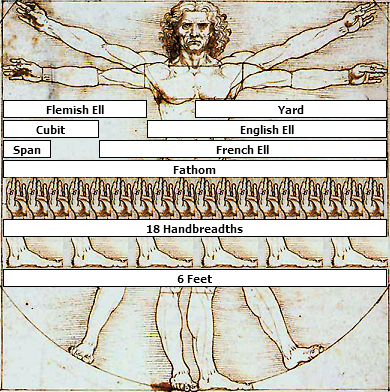
\includegraphics[width=0.7\textwidth]{./graphics/vitruvian-man}

\caption{The Vitruvian Man is a world-renowned drawing created by Leonardo da Vinci around the year 1487.[1] It is accompanied by notes based on the work of the famed architect, Vitruvius. The drawing, which is in pen and ink on paper, depicts a male figure in two superimposed positions with his arms and legs apart and simultaneously inscribed in a circle and square. The drawing and text are sometimes called the Canon of Proportions or, less often, Proportions of Man. It is stored in the Gallerie dell'Accademia in Venice, Italy, and, like most works on paper, is displayed only occasionally.
The drawing is based on the correlations of ideal human proportions with geometry described by the ancient Roman architect Vitruvius in Book III of his treatise De Architectura. Vitruvius described the human figure as being the principal source of proportion among the Classical orders of architecture. Other artists had attempted to depict this concept, with less success. Leonardo's drawing is traditionally named in honor of the architect.}

\end{figure}

According to Leonardo's preview in the accompanying text, written in mirror writing, it was made as a study of the proportions of the (male) human body as described in Vitruvius:

\begin{description}
\item [palm] is the width of four fingers

\item [foot] is the width of four palms

\item [cubit] is the width of six palms

\item [pace] is four cubits

\item [height] a man's height is four cubits (and thus 24 palms)
\end{description}



\subsection{Cubit}
A cubit is the perhaps the first recorded unit of length and was one of many different standards of measurement used through history. It was originally based on measuring by comparing to one's forearm length.

\begin{figure}
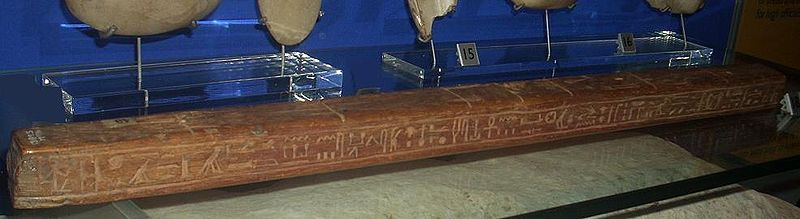
\includegraphics[width=0.9\textwidth]{./graphics/egyptian-cubit}
\caption{Egyptian cubit rule of 0.52m (Liverpool Museum)}
\end{figure}

Cubits were employed through Antiquity, the Middle Ages up to the Early Modern Times, especially for measuring cords and textiles, but also for timbers, stone and volumes of grain.

The Egyptian hieroglyph for the unit shows the symbol of a forearm, but it was rather longer than any actual forearms. The Egyptian cubit was not subdivided into centimetres or inches, but into palms and digits. The Egyptian cubit was subdivided into 7 'palms' of 4 'digits', making 28 parts in all, and was between 52.3 and 52.4cm in length

The English cubit 45.72cm or 457.2mm

\SetConversion{EGcubit}{mm}{525} %varies 523-525mm
\SetConversion{UKcubit}{mm}{457.2}
\SetConversion{EGcubit}{EGpalm}{7}
\SetConversion{EGpalm}{EGdigit}{4}

\FPdiv\tempi{457.2}{525}
\SetConversion{UKcubit}{EGcubit}{\tempi}

\Convert*{1.1234567}{EGcubit}{UKcubit}

It is interesting to note that the Egyptian Royal cupit was related to the diagonal  and $\sqrt{2}R$ = \SI{523,75}{mm}

\begin{marginfigure}
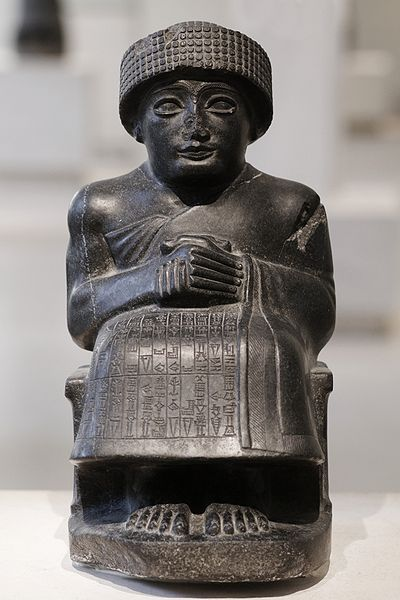
\includegraphics[width=\linewidth]{./graphics/gudea}
\caption{Gudea of Lagash, diorite statue found at Telloh (Louvre)}
\end{marginfigure}
The cubit of King Gudea of Lagash (an ancient Mesopotamian city-state) was 500 mm (19.68 inches). In ancient Israel during the First Temple period, one cubit was 428 mm. During the Second Temple period, an Egyptian cubit of 450 mm was in general use, but in the sacred areas of the temple another cubit of 437 mm was used. (See Biblical Archaeology Review, March-April 1983, and Newsletter and Proceedings of the Society for Early Historical Archaeology, issue 159.)

\subsection{The foot}
And from the forearm the next body part that could be useful was the foot. The foot as a unit of measure was used in most Western cultures and was usually divided into 12 or sometimes 10 inches/thumbs, or into 16 fingers/digits. The first known standard foot measure was from Sumer, where a definition is given in a statue of Gudea of Lagash from around 2575 BC. Some metrologists speculate that the imperial foot was adapted from an Egyptian measure adapted by the Greeks (the ποῦς or pous of between 296 mm and 330 mm) which subsequently became a more consistent measure (the pes of 296 mm) under the Romans.

Effective July 1, 1959 the length of the international yard in the United States and countries of the Commonwealth of Nations was defined as 0.9144 meters. Consequently, the international foot is defined to be equal to exactly 0.3048 meters (equivalent to 304.8 millimeters). This was 2 ppm shorter than the previous U.S  definition and 1.7 ppm longer than the previous British definition.[2]
The international standard symbol for a foot is ``ft'' (see ISO 31-1, Annex A).

\SetConversion{ft}{m}{0.3034}

\convert{0.3034}{m}{ft}\\
\convert{1}{m}{ft}\\

\test{ft}{m}


\chapter{Roman Units}
The ancient units of measurement were built upon the Greek system with influences from Egyptian, Hebrew and Mesopotamian influences. The Roman units were
comparatively consistent and well documented.

\subsection{Lengths}

\begin{marginfigure}
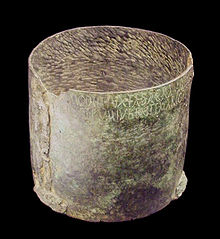
\includegraphics[width=\linewidth]{./graphics/modius}
\caption{Bronze modius measure (4th cent. AD) with inscription acknowledging Imperial regulation of weights and measures.}
\end{marginfigure}

\SetConversion{pes}{ft}{0.967}
\SetConversion{pes}{in}{294.7}

\SetConversion{digitus}{mm}{18.5}

\SetConversion{uncial}{inch}{0.971}


\convert{1}{uncial}{inch} or 
\convert{1}{inch}{uncial}


\SI{4.38}{\square\meter}
\end{document}



\newthought{Bologna}

We are told that the Bologna foot was 0.3805 metres or 14.99 inches; thus 80 Feet of Bologna= 99 English Feet

\SetConversion{Bologna Feet}{inches}{14.99}
\test{Bologna Feet}{inches}


Cloth we learn was sold in Ell or Braccio. 
\SetConversion{Braccio}{m}{0.6350}

\test{Braccio}{m}


\newthought{Dutch foot}

Many countries had their own standard. For example in the Netherlands the \textit{voet} was widely used and was equal to \SI{31}{cm}. Even within the Netherlands the value of the voet varied from area to area. The most commonly use \textit{voet} was the Rijnland foot which was equal to 31.4 cm and had 12 Rijjnland inches. Today the word voet is not in common use in the Netherlands as a unit of measurement. It refers mainly to the "foot" used in English-speaking countries.

\SetConversion{NLft}{m}{0.314}
\SetConversion{Bloois foot}{cm}{30.1}

\test{Bloois foot}{cm}




\subsection{Chain}
\begin{marginfigure}
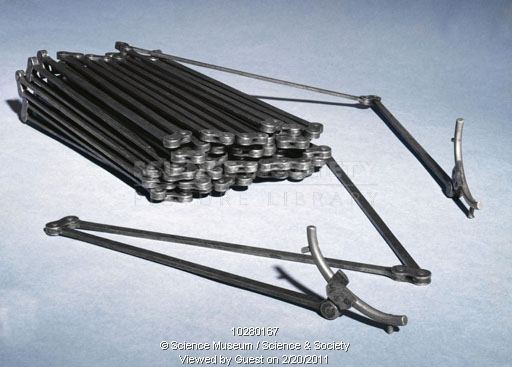
\includegraphics[width=\linewidth]{./graphics/chain}
\caption{100 link steel surveying chain, 1784.
Made by Jesse Ramsden, this chain was used in the Primary Triangulation of Great Britain. This was a network of measured triangles across the country, used to underpin maps. The network was checked in a number of places by setting up a base line, several miles long, and comparing measured and calculated dimensions. The first line was on Hounslow Heath and General William Roy of the Royal Engineers used this chain for its measurement. \url{http://www.scienceandsociety.co.uk/results.asp?image=10280167&wwwflag=2&imagepos=6}}
\end{marginfigure}
The chain has been used for several centuries in Britain and in some other countries influenced by British practice. It was commonly used with the mile to indicate land distances and in particular in surveying land for legal and commercial purposes.


\SetConversion{chain}{yard}{22}
\SetConversion{chain}{ft}{66}
\SetConversion{chain}{link}{100}
\SetConversion{chain}{m}{20.1168}
\SetConversion{engineer's chain}{ft}{100}

\convert{10}{chain}{m}\\
\convert{\outUnitsValue}{m}{chain}\\

\convert{1}{engineer's chain}{ft}


\subsection{Greek Lengths}
Greek measures of length were based on the relative lengths of body parts, such as the foot and finger segment. The specific values assigned to these units varied according to location and epoch (e.g., in Aegina a foot or pous was approximately 13 inches or 333 mm, whereas in Athens (Attica) it was about 11.6 inches or 296 mm).[1] The relative proportions, however, were generally the same throughout the Greek world.

Units derived from the dactylos (plural: dactyloi):

\SetConversion{pous}{mm}{296}
\SetConversion{pous}{inch}{11.6}
\SetConversion{pous}{daktyloi}{16}

\convert{1}{pous}{daktyloi}\\
\convert{1}{pous}{mm}\\

All larger units were derived from the pous (plural: podes)

\SetConversion{diploun bema}{pous}{2.5}% single pace

\convert{1}{pous}{diploun bema}%

Perhaps one of the most common of all was the stadion, which was equal to 600 podes.

\SetConversion{stadion}{pous}{600}
\SetConversion{stadion}{km}{.185}
\SetConversion{EGstadion}{km}{.1575}

The most famous of all calculations using stadia was that of Eratosthenes who measured the circumference of the earth. Based on the interpretation of the length of the stadion, being either the Egyptian at 157.5 meters or the Greek which was 185 meters his calculation was fairly accurate.

Eratosthenes calculation of the circumference of the earth:

(based on Greek stadion) \convert{252000}{stadion}{km}\\

or Egyptian

\convert{252000}{EGstadion}{km}\\

This would give the radius of the earth as:

\FPdiv\radiusi{\outUnitsValue}{\FPpi}\FPdiv\radiusi{\radiusi}{2}

\SI{\radiusi}{\meter}

\SetConversion{m}{km}{0.001}
\convert{\radiusi}{m}{km}

This can be compared to the mean earth radius of 6371 km



\section{More Examples}

\noindent

%% Area\



\test{ft2}{m2}

\convert{11}{ft2}{m2}\\





\test{acres}{km2}



\Rule

\SetConversion{hectare}{m2}{10000}

\test{hectare}{m2}

%% LENGTH
%% 
\SetConversion{inches}{mm}{25.4}

\test{inches}{mm}

\Rule



\SetConversion{Angstrom}{m}{0.0000000001}

\Rule

%% ASTRONOMICAL UNIT OF LENGTH
\SetConversion{Au}{km}{149597870.700}
\convert{149597870.700}{km}{Au}\\
\convert{1}{Au}{km}\\

\Rule

\SetConversion{lightyear}{Au}{63241}
\convert{63241}{Au}{lightyear}\\

\Rule




\section{Nautical Dimensions}

%% Nautical mile

\SetConversion{NM}{ft}{6076.1155}
\convert{1}{NM}{ft}\\
\convert{6000}{ft}{NM}\\


\SetConversion{NM}{yard}{2025.372}
\convert{1}{NM}{yard}\\
\convert{1}{yard}{NM}\\


\SetConversion{NM}{equatorialarcminute}{0.998383}
\SetConversion{NM}{meridianarcminute}{0.998383}

\Rule

\SetConversion{NM}{m}{1852}%nautical mile
\convert{1}{NM}{m}\\
\convert{1852}{m}{NM}\\

\Rule

\SetConversion{NM}{fathom}{1012.6859}
\convert{1}{NM}{fathom}\\
\convert{1012.6859}{fathom}{NM}\\

\Rule
%%% Volume
%%%



\SetConversion{ft3}{m3}{0.028316846592}

\Rule

\convert{10}{ft3}{m3}\\
\convert{1}{m3}{ft3}\\


%%% Volume Imperial
\SetConversion{gallon}{pint}{8} %Imperial ounce

\convert{8}{pint}{gallon}\\

\SetConversion{gallon}{oz}{160}
\SetConversion{gallon}{ounce}{160}
\SetConversion{quart}{ounce}{40}




\SetConversion{teaspoon}{m3}{.000017758 164 0625}
\SetConversion{cfm}{lpm}{2}
\SetConversion{atm}{Pa}{10325}
\SetConversion{BTU}{J}{1054.500}
\SetConversion{hp}{W}{746}
\SetConversion{GPM}{m3persec}{0.0000630901964}

%% Time

\SetConversion{Day}{s}{86164.1}


%% Frequency

\SetConversion{rpm}{radpersec}{0.104719755}

%% Speed or velocity

\SetConversion{fpm}{mpersec}{.00508}
\SetConversion{fpm}{m/s}{.00508}
\SetConversion{knots}{km/h}{1.852}

\Rule

\SetConversion{knot}{ft/s}{1.687810}

\convert{1}{ft/s}{knot}\\
\convert{1}{knot}{ft/s}\\

\Rule

%%% Temperature


%\SetConversion{C}{K}{273.15}
\def\CtoK#1{\FPadd\result{#1}{273.15}%
\FPround\result{\result}{2}%
\sisetup{
fixed-exponent = 2,
scientific-notation = false}
 \num{\result}}


%% Convert Centigrate to Fahreneit
\def\CtoF#1{\FPdiv\resulta{9}{5}%
\FPmul\resultb{\resulta}{#1}%
\FPadd\resultc{\resultb}{32}%
\FPround\resultc{\resultc}{3}%
 \num{\resultc}%
\sisetup{
fixed-exponent = 0,
scientific-notation = false}
}

%% Convert Fahreneit to Centigrade
\def\FtoC#1{\FPdiv\resulta{5}{9}%
\FPsub\resultb{#1}{32}%
\FPmul\resultc{\resultb}{\resulta}%
\FPround\resultc{\resultc}{\numdec}%
\sisetup{
fixed-exponent = 0,
scientific-notation = false}
\num{\resultc}%
}

%% Convert Fahreneit to Rankine
\def\FtoRa#1{\FPmul\result{#1}{9}%
\FPdiv\result{\result}{5}%
\FPround\result{\result}{\numdec}%
\result%
}

%% Convert Kelvin to Rankine
\def\KtoRa#1{\FPadd\result{#1}{459.67}%
\FPround\result{\result}{\numdec}\result}

%% Convert Rankine to Celcius
\def\RtoC#1{\FPsub\result{#1}{459.67}% to fahreneit
\FtoC{\result}}

%% Mass 
\SetConversion{grain}{g}{0.06479891}

\convert{1}{grain}{g}\\
\convert{1}{g}{grain}\\

\Rule



\SetConversion{grain}{mg}{0.06479891}
\SetConversion{drachm}{g}{1.7718451953125}
\SetConversion{drc}{g}{1.7718451953125}
\SetConversion{lb}{kg}{0.45359237}
\SetConversion{st}{kg}{6.35029318}
\SetConversion{stone}{kg}{6.35029318}
\SetConversion{cwt}{lb}{112}
\SetConversion{hundredweight}{lb}{112}
\SetConversion{ton}{lb}{2240}

%% Acceleration

\SetConversion{lb}{N}{4.448230531}
\SetConversion{lbf}{N}{4.4482216152605}




\global\def\numdec{5}


%%% Pressure or mechanical stress

\SetConversion{atm}{Pa}{101325}
\convert{100000}{Pa}{atm}\\

\Rule

\SetConversion{atm}{kPa}{101.325}


\convert{100000}{kPa}{atm}\\
\convert{1}{atm}{kPa}\\

\Rule


\SetConversion{bar}{kPa}{101.325}
\SetConversion{bar}{Pa}{100000}

%% Conversion needs checking
\SetConversion{mmHg}{Pa}{133.3224}
\SetConversion{mmH2O}{Pa}{9.80638}
\SetConversion{Pa}{mmHg}{0.01}

\SetConversion{inH2O}{Pa}{249.082}
%% See write-up as to where Torr is used.
\SetConversion{torr}{Pa}{133.3224} 


\SetConversion{torr}{mmHg}{0.999999857533699}

\expandafter\def\csname mmH2O\endcsname{mmH$_2$O}
\expandafter\def\csname inH2O\endcsname{inH$_2$O}

\Rule

\convert{12}{mmHg}{Pa}\\
\convert{1}{Pa}{mmHg}\\
\convert{100}{mmH2O}{Pa}\\
\convert{980.64}{Pa}{mmH2O} (Error!)\\

%% Non-sense units
\SetConversion{m3/s/m3}{ft3/lb/s}{10}

\convert{10}{m3/s/m3}{ft3/lb/s}\\
\convert{10}{ft3/lb/s}{m3/s/m3}\\

\Rule

%% Calories
%% We have the small and the large calorie

\SetConversion{cal}{J}{4.184} % Thermochemical calories
\SetConversion{cal15}{J}{4.1855}
\expandafter\def\csname cal15\endcsname{cal$_{15}$}
\expandafter\def\csname note-cal15\endcsname{measured at 15 deg C}

\convert{100}{cal15}{J}\sidenote{\csname note-cal15\endcsname}\\
\convert{100}{J}{cal15}\\


\medskip

\SetInBetween{&$\to$&}
\begin{tabular}{lll}
\toprule
\convert{1}{Pa}{mmHg}\\
\convert{1}{mmHg}{Pa}\\
\convert{1}{bar}{Pa}\\
\convert{1}{kPa}{bar}\\
\bottomrule
\end{tabular}


\newenvironment{conversiontable}{%
\SetInBetween{&$\to$&}
\begin{tabular}{lll}
\toprule
}{%
\bottomrule
\end{tabular}
}




\SetInBetween{equals}
\num{3.45d-4}

\SIlist{10;23;45}{\meter}\\

\Rule

Temperatures

\begin{conversiontable}
  \convert{100}{C}{K}\\
  \convert{100}{C}{F}\\
  \convert{300}{C}{F}\\
  \convert{212}{F}{C}\\
  \convert{212}{F}{Ra}\\
  \convert{212}{K}{Ra}\\
  \convert{459}{R}{C}\\
\end{conversiontable}





\SetInBetween{ = }

\makeatother

\chapter{Weights}

The avoirdupois is a system of weights (or, properly, mass) based on a pound of sixteen ounces. It is the everyday system of weight used in the United States, and is still widely used to varying degrees by many people in Canada, the United Kingdom, and some other former British colonies despite the official adoption of the metric system. An alternate system of mass is generally used for precious materials, Troy weight.

\begin{figure}[p]
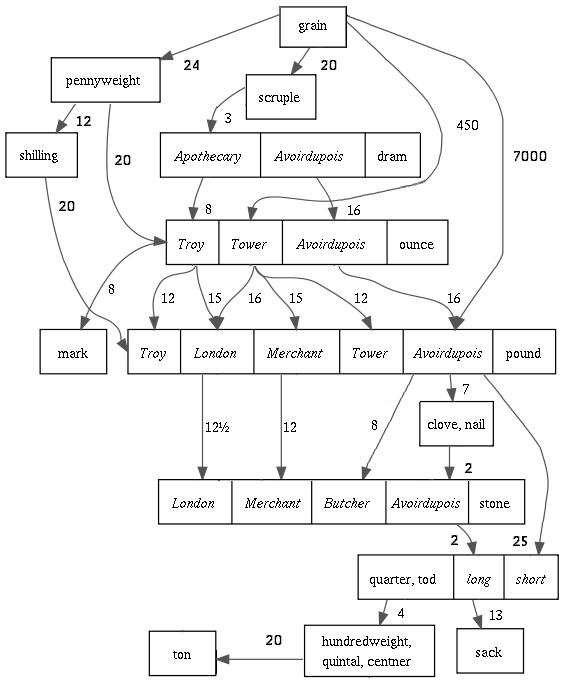
\includegraphics[width=1.2\linewidth]{./graphics/englishweights}
\caption{Chart showing the relationships of English weight measures.}
\end{figure}

When people in the United Kingdom began to use this system they included the stone, which was eventually defined as fourteen avoirdupois pounds. The quarter, hundredweight, and ton were altered, respectively, to 28 lb, 112 lb, and 2,240 lb in order for masses to be easily converted between them and stones. 





\newthought{Cologne}

In Cologne at the early 1800s, we find that gold and silver were weighted by the Mark of 8 ounces, 16 Loths, 64 Quintins,256 pfenings or Deniers, 4352 Eschen, or 65536 Richtpfenings. The Mark had a weight of 233.769 Grammes or 3608 Grains.\sidenote{The Cologne Mark was, by an edict of the Emperor Charles 5th, in 1524, declared the standard weight for the precious metals throughout Germany, and copies were deposited in the principal cities of the Empire.}

\SetConversion{Mark}{ounce}{8}

\newthought{Copenhagen}

\SetConversion{PoundCopenhagen}{PoundAvoirdupois}{1.1028}
%\expandafter\def\csname PoundCopenhagen\endcsname{Pound$_{\text{Copenhagen}}$}

\SetUnit{PoundCopenhagen}{Pound$_{\text{Copenhagen}}$}
\SetUnit{PoundAvoirdupois}{Pound$_{\text{Avoirdupois}}$}


\convert{100.00}{PoundCopenhagen}{PoundAvoirdupois}


\section{Old Cypriot Units}

\subsection{Old Cypriot Units of Length and Area}
% Setting deefault typesetting
\SetUnit{CYscala}{scala$_{\text{Cypriot}}$}
\SetUnit{CYscala}{scala (Cypriot)}


\SetConversion{pic (Cypriot)}{m}{0.6096}
\SetConversion{pic (Turkish)}{m}{0.755397246487}
\SetConversion{foot (Cypriot)}{m}{0.3048}
\SetConversion{CYscala}{m2}{1337.803776}
\SetConversion{oke}{kg}{1.270058636}


\begin{conversiontable}
\convert{1}{pic (Cypriot)}{m}\\
\convert{1}{pic (Turkish)}{m}\\
\convert{2}{foot (Cypriot)}{m}\\
\Convert*{1.00000}{oke}{kg}\\
\convert{1}{kg}{oke}\\
\convert{1}{CYscala}{m2}\\
\end{conversiontable}

\section{Conversions by multiplication}

Most units can be converted to and from each other by simply multiplying them by a conversion factor.

For example pounds (lb) can be converted to kilograms by multiplying it with the factor 0.453 592 37. The reverse conversion can be achieved by multiplying Kilograms with 1/0.45359237 to obtain the pounds. Most units can be converted in this way. The package provides an easy way to achieve this, by using:

\convert{1}{lb}{kg}

\convert{1}{kg}{lb}


\convert{1}{lbf}{N}

\convert{1}{N}{lbf}

\begin{lstlisting}
 \SetConversion{Unit1}{Unit2}{conversion factor}
\end{lstlisting}

To set the conversion factors from pounds to kilograms and vice versa, you define the following:

\begin{lstlisting}
 \SetConversion{lb}{kg}{0.45359237}
\end{lstlisting}

To convert a 10 pound to kilograms,

\begin{lstlisting}
 \convert{10}{lb}{kg}
\end{lstlisting}

You have available two commands when you define a conversion this way:

\begin{lstlisting}
 \lbtokg
 \kgtolb
\end{lstlisting}

\section{Notes on the User Interface}

I have tried to keep the user interface as simple as possible. The user need only use one macro for most cases to effect a conversion.

\begin{lstlisting}
 \convert{10}{lb}{kg}
\end{lstlisting}

The unit names are those commonly found in various scientific fields, as well as commonly used in the US (for Imperial Units). In addition units that are difficult to remember their symbol, you can use both their full name or a symbol, for example:

\convert{2}{quart}{ounce}

\convert{2}{gallon}{oz}

Most common units can be found pre-built. For example it is customaty that pump pressure is measured in kPa, rather than Pa, so if you type

\convert{5.20}{atm}{kPa}, whereas \verb+\convert{5}{mmHg}{Pa}+ will produce \convert{5}{mmHg}{Pa}.

There is a setting out command called \verb+\SetInBetween+ 

\SetInBetween{$=$}

\convert{1213.67}{lb}{kg}

\SetInBetween{$\rightarrow$}

\convert{1213.67}{lb}{kg}

\SetInBetween{equals}

\convert{1213.67}{lb}{kg}

\convert{30}{knots}{km/h}




\subsection{New units}

The package provide conversion factors for over a thousand units. This includes, ancient, historical and modern units. If one is missing, you can add a new one by using,

\begin{verbatim}
\SetConversion{lb}{kg}{conversion factor}
\end{verbatim}

When you define conversion formulae as above, the package provides a two way conversion, i.e, you only need to set the conversion factor once.


For units that cannot be converted by a multiplication factor alone, a macro must be written for the conversion. For example the built-in macro to convert degree Fahreneit to Centigrate is defined as follows:

\begin{verbatim}
%% Convert Fahreneit to Centigrade
\def\FtoC#1{\FPdiv\resulta{5}{9}%
\FPsub\resultb{#1}{32}%
\FPmul\resultc{\resultb}{\resulta}%
\FPround\resultc{\resultc}{\numdec}%
\sisetup{
  fixed-exponent = 0,
  scientific-notation = false}
\num{\resultc}%
}
\end{verbatim}




\section{Conventions}

Many units have the same name, but have different values in different geographical areas. For example we have the British pound and the Italian pound. I have used the country code as a prefix. For example, the greek stadion can be compared to the Egyptian stadion using

\begin{verbatim}
\convert{1}{stadion}{EGstadion}
\end{verbatim}

A better approach is to use it as a subscript?

\SetConversion{stadion-greek}{m}{185}
\convert{3}{stadion-greek}{m}






\section{convertresult}

The conversion results can be used so that they can be manipulated further. They are stored in \verb+ \convertresult+


\section{Typesetting the units}

The package automatically detects if the \texttt{siunitx} is loaded. If it is not loaded it will be loaded automatically. The is unit developed and maintained by Joseph Wright is used to typeset most of the SI units.

\section{Formatting Numbers}

You can format a number in a variety of ways:

\verb+\FormatNumber[7]{-1.345678000000000}+

\FormatNumber[5]{3.28976756}

This will format the number to 7 decimal places. In addition any redundant zeroes will be clipped, if the option clip=true is set.

\section{options}

clip=true  clip redunandant zeroes

decimals=2 sets globally all numbers to be to two decimal places

\section{Conversion Tables}

The command

\begin{description}

\item \verb+\converttable{area}+ will produce a table of all the conversion factors available for areas.

\item \verb+\converttable{length}+ will produce a table all the conversion factors available for lengths. 

\item \verb+\converttable{weight}+ will produce a table of all the conversion factors for weights.

\end{description}



%
%\def\foo{test}
%
%
%\ifcsname CK\endcsname
%  {\csname \foo\endcsname\space is defined}%
%\else
%  {no command \string\m2}%
%\fi
%
%
%%% Numprint commands
%%% 
%
%\numprint{-e4.3242}, \numprint{+-e4.3242} 
%
%\textdegree K

\chapter{Pressure units}
\begin{marginfigure}
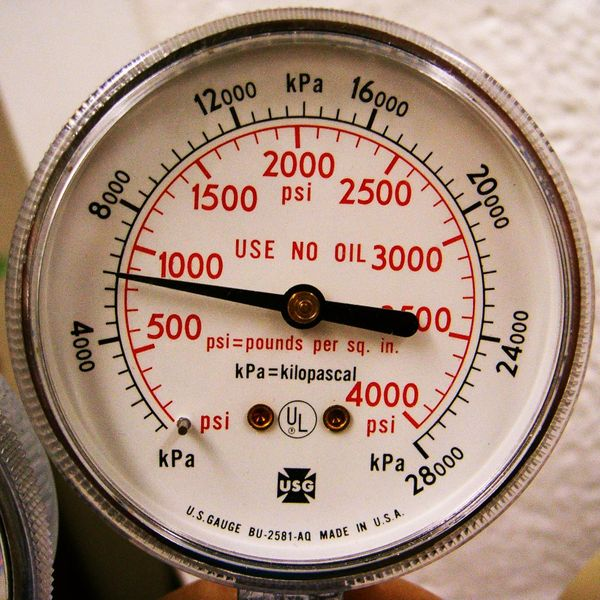
\includegraphics[width=\linewidth]{./graphics/pressuregauge}
\end{marginfigure}



The internationally recognised SI unit for pressure is the pascal, abbreviated to Pa, and this is the unit realised by the primary measurement standards in the world's national metrology institutes to provide traceability for pressure measurements.

There are many other pressure units in service - indeed pressure has more units than most subjects and it is usually assumed that to convert from one to another all that is needed is the right conversion factor. 

For example \SI{1}{mbar} equals 100 pascals; 1 bar equals 100 000 pascals or 1 kilogram-force per square centimetre (kgf/cm2) equals the not-so-round-number of 98 066.5 pascals. The conversion factors in these examples are EXACT - no amount of computing will produce another decimal place. But not all conversions are or can be expressed exactly because their definitions are incompatible with the definition of the pascal. Use of certain pressure units guarantees the introduction of conversion errors and increases the chance of confusion-induced mistakes.



The problematical units include those known as manometric units - which define pressure in terms of the length of liquid column at a specified (but non-realisable) density - and include all those using two of the words: inches, feet, millimetres, centimetres, mercury, water, oil or their abbreviations, for example millimetres of mercury (mmHg). In short, it is the need to assume fixed and exact but ultimately incorrect values of liquid density and acceleration due to gravity that inherently limits knowledge of the relationship between these units and the pascal. By contrast, the magnitude of pressure values expressed in the SI pressure unit, the pascal, can flex (albeit not by much) to take account of technological improvements in the underlying definitions of mass, length and time - the SI base quantities from which pressure is derived.




\subsection{Torr}

The torr (symbol: Torr) is a non-SI unit of pressure with the ratio of 760 to 1 standard atmosphere, chosen to be roughly equal to the fluid pressure exerted by a millimeter of mercury, i.e. a pressure of 1 Torr is approximately equal to 1 mmHg. Note that the symbol is spelled exactly the same as the unit, but the symbol is capitalized, as is customary in metric units derived from names. It was named after Evangelista Torricelli, an Italian physicist and mathematician who discovered the principle of the barometer in 1644.

The torr (symbol: Torr) is a non-SI unit of pressure with the ratio of 760 to 1 standard atmosphere, chosen to be roughly equal to the fluid pressure exerted by a millimeter of mercury, i.e. a pressure of 1 Torr is approximately equal to 1 mmHg. Note that the symbol is spelled exactly the same as the unit, but the symbol is capitalized, as is customary in metric units derived from names. It was named after Evangelista Torricelli, an Italian physicist and mathematician who discovered the principle of the barometer in 1644.

\subsection{millimetre of mercury}
In medicine, the millimetre of mercury (measured with a sphygmomanometer) is the "gold standard" for blood pressure measurement.

In physiology, manometric units are used to measure Starling forces. Other applications include:

\begin{enumerate}
\item Intraocular pressure (tonometry)
\item Cerebrospinal fluid pressure
\item Intracranial pressure\sidenote{Intracranial pressure (ICP) is the pressure inside the skull and thus in the brain tissue and cerebrospinal fluid (CSF). The body has various mechanisms by which it keeps the ICP stable, with CSF pressures varying by about 1 mmHg in normal adults through shifts in production and absorption of CSF. CSF pressure has been shown to be influenced by abrupt changes in intrathoracic pressure during coughing (intraabdominal pressure), valsalva (Queckenstedt's maneuver), and communication with the vasculature (venous and arterial systems). ICP is measured in millimeters of mercury (mmHg) and, at rest, is normally 7-15 mmHg for a supine adult, and becomes negative (averaging −10 mmHg) in the vertical position.[1] Changes in ICP are attributed to volume changes in one or more of the constituents contained in the cranium.
Intracranial hypertension, commonly abbreviated IH, is elevation of the pressure in the cranium. ICP is normally 7-15 mm Hg; at 20-25 mm Hg, the upper limit of normal, treatment to reduce ICP is needed.}
\item Intramuscular pressure (compartment syndrome)
\item Central venous pressure
\item Pulmonary artery catheterization
\item Mechanical ventilation
\end{enumerate}

Manometric results in medicine are sometimes given in torr.
This is usually incorrect, since the torr and the millimetre of mercury are not the same thing.
Pressures obtained with a manometer (or its transducer equivalent) should be reported in millimetres of mercury.

The unit mmHg as used in medicine is in general given relative to the atmospheric pressure. This means that when a doctor tells you you have a blood pressure of 100 mmHg, this is 100mmHg above atmospheric. So on a day when the barometric pressure is 760 your absolute pressure is actually 760 + 100 = 860 mmHg = $860/760\times105$Pa. \numdec{10}\convert{130}{torr}{mmHg}




\chapter{Formatting the Output}

\si{\cubic\lux\volt\tesla\cubed}
\subsection{Tabular material}

\begin{table}
\caption{Standard behaviour of the \texttt{S} column type.}
\label{tab:S:standard}
\centering
\begin{tabular}{S}
\toprule
{Some Values} \\
\midrule
2.3456 \\
34.2345 \\
-6.7835 \\
90.473 \\
5642.5 \\
1.2e3 \\
e4 \\
\bottomrule
\end{tabular}
\end{table}

\ang{6;7;6.5} \\

 \si{\metre\second} = \text{metre second}  \\
 \si{\milli\second} = \text{millisecond}  \\

\sisetup{inter-unit-separator = { } . { } }

 \si{\metre\second} = \text{metre second} 

 \si{\milli\second} = \text{millisecond} 

\convert{13.2345}{ft2}{m2}


$\SI{13.45678}{\si{mmHg}}$




\makeatletter

%% The command SetPlural saves the plurals
%% for a particular unit

\newcommand\SetPlural[3]{
\expandafter\gdef\csname plural@#1\endcsname{#2}%
\expandafter\gdef\csname pluralp@#1\endcsname{#3}%
}


%% We use the suffix package to simplify the code
%% between starred and non-starred versions of commands

\newcommand\plural[2][]{\SI{#1}{%
\csname pluralp@#2\endcsname}}%

\WithSuffix\newcommand\plural*[2][]{\SI{#1}{\csname plural@#2\endcsname}}



\SetPlural{kg}{kgs}{kilogrammes}
\SetPlural{ft}{ft}{feet}
\SetPlural{gm}{gms}{grams}




\chapter{Plurals and Singulars}

Measures such as the foot, when used inline with a number must be in plural. It is better to say \plural[13]{ft} rather than \SI{13}{ft} and certainly a `thirteen foot length' is wrong.

The package provides commands that enable the saving and re-use of plurals.
This is especially useful if you set the options to verbose.

\begin{verbatim}
\usepackage[verbose=auto,decimals=2]{convert}
\end{verbatim}

If the option verbose is set to auto, all conversion typesetting will be in the plural if the units convert to a number greater than one.



\newthought{Example}

Consider that \plural[2000]{gm} is equal to two kilogrammes. 




\section{Humanize}

The package also provides limited means to provide the full names of units, as well as to provide plurals.

\begin{verbatim}
\plural*{kg}
\end{verbatim}

\noindent will give you

\noindent \texttt{> kgs}

To set it you can use the command

\begin{verbatim}
\SetPlural{kg}{kgs}{kilogrammes}
\SetPlural{CYPound}{lbs (Old Cypriot)}{Pounds (Old Cypriot)}
\end{verbatim}






The starred version

\plural*[57]{kg}

The plain version of the command

\plural[57]{kg}

\SetPlural{oz}{oz}{ounces}

\plural[6]{oz} 



\plural[13]{ft}




\section{Notes and help}

\long\def\makenote#1#2{%
\expandafter\def\csname cs@note#1\endcsname{#2}}

\makenote{oz}{There are 16 ounces in a pound.}

\def\PrintNote#1{\csname cs@note#1\endcsname}
This is a\sidenote{\PrintNote{oz}} footnote



\chapter{Conversion Tables}
For convenience units are tabulated in conversion tables as shown in Table~\ref{tbl:converttable1}. A conversion table such as this provides 70 conversion values, i.e., you can convert between mile to meters and from meters to mile.

\bigskip
\def\z{\phantom{0}}
%% Typesetting the stepped tabular table
%% The table is typeset as stepped up to enable 
%% ease of reading
%%
% The maximum number of cells must be given for calculation
\gdef\maxcell{9}
% We define a counter to step up the row counts
% automatically
\newcounter{rcount}
\setcounter{rcount}{0}
% helper routine
\gdef\row#1{\addtocounter{rcount}{1}#1\\\cline{\thercount-\maxcell}}
%% The typical row is defined with a multicolumn at the front
%% to enable the step
\gdef\Row#1{\multicolumn{\thercount}{r|}{}\row{#1}}
%% The first row is a special case we need the first cell to be in
%% |r|
\gdef\Ron#1{\multicolumn{\thercount}{|r|}{1\z}\row{#1}}
%% The heading 
\gdef\TopRow#1{\hline#1\\
\hline}

%% Setting the first row
%%
\FPset\xi{8\z}
\FPset\xii{320\z}
\FPset\xiii{1760\z}
\FPset\xiv{5280\z}
\FPset\xv{63360\z}
\FPset\xvi{190080\z}
\FPset\xvii{1609.3059}

%% Set the conversion factors
\SetConversion{furlong}{pole}{40}
\SetConversion{furlong}{yard}{220}
\SetConversion{furlong}{ft}{660}
\SetConversion{furlong}{inches}{7920}
\SetConversion{furlong}{barley corn}{23760}
\SetConversion{furlong}{meter}{201.1632}
%% Pole
\SetConversion{pole}{yard}{5.5}
\SetConversion{pole}{feet}{16.5}
\SetConversion{pole}{inches}{198}
\SetConversion{pole}{barley corn}{594}
\SetConversion{pole}{meter}{5.0291}
%% Yard
\SetConversion{yard}{ft}{3}
\SetConversion{yard}{inches}{36}
\SetConversion{yard}{barley corn}{108}
\SetConversion{yard}{meter}{0.9144}
%% Feet
\SetConversion{ft}{inches}{12}
\SetConversion{ft}{barley corn}{36}
\SetConversion{ft}{meter}{0.3048}
%% Inches
\SetConversion{inches}{barley corn}{3}
\SetConversion{inches}{meter}{0.0254}
%% barley corn
\SetConversion{barley corn}{meter}{0.0085}

\begin{fullwidth}
\begin{table}[htbp]
\vspace{0.9cm}
\begin{tabular}{|r |r |r |r |r |r |r |l r|}
\TopRow{Mile &Furlong&Pole &Yard\z &Feet\z &Inches &Barley Corns &&Meters}
\Ron{&\xi &\xii    &\xiii  &\xiv &\xv &\xvi &=&\xvii}
\Row{&1\z &\furlongpole\z &\furlongyard\z&\furlongft\z &\furlonginches\z &23760\z &=&\furlongmeter}
\Row{&1\z &$5\frac{1}{2}$ &$16\frac{1}{2}$   &198\z &594\z &=&5.0291}
\Row{&1\z &3\z   &36\z  &108\z &=&0.9144}
\Row{&1\z &12\z  &36\z &=&0.3048}
\Row{&1\z &3\z &=&0.0254}
\Row{&1\z &=&0.0085}
\end{tabular}
\caption{Conversion table for traditional english units of length.}
\end{table}
\label{tbl:converttable1}
\end{fullwidth}

It will be nice if the package provides some means to provide an interface for such tables.

\begin{eqnarray}
t_1=f\cdot t_2 \\ 
t_2=\frac{1}{f}\cdot t_1
\end{eqnarray}

We do not need to provide all the interconnected values, we only need to provide the first row of the conversion factors. The program can then calculate the others.

As for example to get the conversion factor $f$ for converting inches to meters, we can get it from the first row fo the table as follows\sidenote{Values shown are as calculated using  the fp package.}:

\begin{eqnarray}
              f &=&\frac{1609.3059}{63360}\\[10pt] 
              &=& \FPdiv\tmp{1609.3059}{63360}\tmp\\
              &=& \SI{0.0254}{\meter\per in}
\end{eqnarray}

To convert in the opposite way we just invert the calculation:


\begin{eqnarray}
            f &=&\frac{63360}{1609.3059}\\[10pt] 
              &=& 39.3710\\
              &=& \SI{39.3710}{in\per\meter}
\end{eqnarray}

There many possible ways to develop both the datastructure as well as the interface. The easiest would be to provide simple macros with up to the maximum delimiters possible. Another way is to have a variable number of arguments or use a comma delimited list. First let us use a simple macro:


\begin{verbatim}
\long\def\GetUnits#1#2#3#4#5#6#7#8#9{
\begin{tabular}{lllllllll}
\hline
#1 #2 #3 #4 #5 #6 #7 #8\\
\hline
\end{tabular}
}
\end{verbatim}






%% Helper routine for formatting numbers
%% first it round to 4 decimal numbers
%% then it clips the number so that if trailing
%% zeroes exist it removes them prints 16.01 and not 16.010000000
%% usefull for conversion table will show 12 inches not 12.0000
%% Clip round and clip
%% Clip* round Clip and put an equal sign at the front
\newcommand\Clip[1]{\FPround\tmp{#1}{3}\FPclip\tmp{\tmp}$\tmp$}%
%
%% The starred version of the command
\WithSuffix\newcommand\Clip*[1]{%
\FPround\tmp{#1}{4}\FPclip\tmp{\tmp}%
$=\tmp$}%
%
%% Helper macros
%% Checks that arguments are not empty
%% If empty returns nothing
%% To do check for second argument if zero
\newcommand\CF[4][]{%
%% let the \#1 be empty easier
%% for letting it to empty when
%% the conditionals reject it for being empty
\def\@empty{}%
\expandafter\gdef\csname#1\endcsname{}%
%% we globally set \varone and \vartwo to enable
%% checking with the FPifgt
\gdef\varone{#3}%
\gdef\vartwo{#4}%
\gdef\zero{0}%
\def\IsEmpty{#3}%
\ifx\varone\@empty% argument 1 is empty%
  \else% 
    \ifx\vartwo\@empty% argument 2 is empty% 
      \else%
        \expandafter\gdef\csname#2\endcsname{%
          \FPifgt\vartwo0\FPdiv\tmp{#3}{#4}%
             \Clip#1{\tmp}%\Clip#1{
          \else%
         \fi}%
     \fi%
\fi}%
%% We define the units here we also build the units
\gdef\GetUnits#1#2#3#4#5#6#7#8{%
%% We create globals to hold the input variable names
%% We use these later to create a set of SetConvert for all the units
%% and have a one to one relationship with the values that are inputted
\expandafter\gdef\csname uniti\endcsname{#1}%
\expandafter\gdef\csname unitii\endcsname{#2}
\expandafter\gdef\csname unitiii\endcsname{#3}
%\global\let\unitsii\unitii%
%\global\let\unitsiii\unitiii%
\expandafter\gdef\csname unitiv\endcsname{#4}%
\expandafter\gdef\csname unitv\endcsname{#5}%
\expandafter\gdef\csname unitvi\endcsname{#6}%
\expandafter\gdef\csname unitvii\endcsname{#7}%
\expandafter\gdef\csname unitviii\endcsname{#8}%
%% These is to just typeset the first row with the units
#1&#2 &#3 &#4 &#5&#6 &#7&#8\\\hline%
}%

%% With this command we define all the ratios for a table with
%% up to eight levels. Longer tables might give problems
\gdef\GetRatios#1#2#3#4#5#6#7#8{%
\Clip{#1}&\Clip{#2}&\Clip{#3}&\Clip{#4}&\Clip{#5}&\Clip{#6}&\Clip{#7}&\Clip*{#8}%ERROR to be corrected
\CF{fthree}{#3}{#2}%
\CF{ffour}{#4}{#2}%
\CF{ffive}{#5}{#2}%
\CF{fsix}{#6}{#2}%
\CF{fseven}{#7}{#2}%
\CF[*]{feight}{#8}{#2}%
%% Third unit
\CF{ffouri}{#4}{#3}%
\CF{ffivei}{#5}{#3}%
\CF{fsixi}{#6}{#3}%
\CF{fseveni}{#7}{#3}%
\CF[*]{feighti}{#8}{#3}%
%% Fourth unit
\CF{ffiveii}{#5}{#4}%
\CF{fsixii}{#6}{#4}%
\CF{fsevenii}{#7}{#4}%
\CF[*]{feightii}{#8}{#4}%
%% Fifth unit
\CF{fsixiii}{#6}{#5}%
\CF{fseveniii}{#7}{#5}%
\CF[*]{feightiii}{#8}{#5}%
%% Sixth unit
\CF{fseveniv}{#7}{#6}%
\CF[*]{feightiv}{#8}{#6}%
%% Seventh unit
\CF[*]{feightv}{#8}{#7}%
%% After a long time managed to get it to
%% 

\gdef\Conversions##1##2##3##4{%
\FPdiv\inverse{##3}{##4}
\global\let\inverts\inverse
\expandafter\gdef\csname##1##2\endcsname{\inverts}%Define one way
%

\FPdiv\inver{##4}{##3}
\global\let\invert\inver
\expandafter\gdef\csname##2##1\endcsname{\invert}
 %\gdef\Test{\csname##2##1\endcsname}
%\csname##1##2\endcsname
 }

%% Furlong to pole
\Conversions{\unitii}{\unitiii}{#3}{#2}
\Conversions{\unitii}{\unitiv}{#5}{#2}%% calculations need correction

%\csname##1##2\endcsname
%\Test

}

\SetInBetween{ =}

%\begin{tabular}{|l|l|l|l|l|l|l|l|}
%\hline
%\GetUnits{$L_1$}{$L_2$}{$L_3$}{$L_4$}{$L_5$}{$L_6$}{$L_7$}{$L_8$}\\
%\cline{1-8}
%\GetRatios{$f_1$}{$f_2$}{$f_3$}{$f_4$}{$f_5$}{$f_6$}{$f_7$}{$f_8$}\\
%\cline{1-8}
%\GetRatios{}{1}{$f_{4}/f_2$}{$f_4/f_2$}{$f_5/f_2$}{$f_6/f_2$}{$f_7/f_2$}{$f_8/f_2$}\\
%\cline{1-8}
%\GetRatios{}{}{1}{$f_4/f_3$}{$f_5/f_3$}{$f_6/f_3$}{$f_7/f_3$}{$f_8/f_3$}\\
%\cline{1-8}
%\GetRatios{}{}{}{1}{$f_5/f_4$}{$f_6/f_4$}{$f_7/f_4$}{$f_8/f_4$}\\
%\cline{1-8}
%\GetRatios{}{}{}{}{1}{$f_6/f_5$}{$f_7/f_5$}{$f_8/f_5$}\\ 
%\cline{1-8}
%\end{tabular}


\bigskip



One interesting observation, is that if we need to add another factor or relationship of length we may not need to construct another table, but just add one other unit. For example we could add Leagues just before the mile and we can have the conversion of Leagues or Nautical miles incorporated into our database.

\bigskip

\index{Tables!stepped table}
Trying our stepped table calculations using the English long units, defining land measurements, we get:
\bigskip

%% We define the stepped rows in a 
%% a convenience macro
\gdef\TypesetSteppedRows{
\hline
\multicolumn{1}{l|}{}&1
  &\fthree
  &\ffour
  &\ffive
  &\fsix
  &\fseven
  &\feight\\
  \cline{2-8}
\multicolumn{2}{l|}{}&1 
  &\ffouri
  &\ffivei 
  &\fsixi
  &\fseveni
  &\feighti \\
\cline{3-8}
\multicolumn{3}{l|}{}&1 
  &\ffiveii 
  &\fsixii
  &\fsevenii
  &\feightii \\
\cline{4-8}
\multicolumn{4}{l|}{}&1 
  &\fsixiii
  &\fseveniii
  &\feightiii\\
\cline{5-8}
\multicolumn{5}{l|}{}&1 
  &\fseveniv
  &\feightiv\\
\cline{6-8}
\multicolumn{6}{l|}{}&1 
&\feightv\\
\cline{7-8}}



%% This will typeset a stepped table
\begin{tabular}{|l|l|l|l|l|l|l|l|}
\hline
\GetUnits{Mile}{Furlong}{Pole}{Yard}{Feet}{Inches}{Barley Corns}{Meters}
\hline
\GetRatios{1}{8}{320}{1760}{5280}{63360}{190080}{1609.3059}\\
\TypesetSteppedRows
\end{tabular}




\convert{1}{Pole}{Furlong}

\convert{1}{Furlong}{Pole}

\convert{1}{Furlong}{Yard}
%% Creating an environment for the users
\newenvironment{converttable}
{\begin{tabular}{|l|l|l|l|l|l|l|l|}
\hline}
{\TypesetSteppedRows
\end{tabular}}


%% Testing the environment
\begin{table}[htbp]
\vspace{1cm}
\begin{converttable}
\GetUnits{Miles}{Furlongs}{Poles}{Yard}{Feet}{Inches}{Barley Corns}{Meters}
\GetRatios{1}{8}{320}{1760}{5280}{63360}{190080}{1609.3059}\\
\end{converttable}
\caption{Old British units of distance.}
\end{table}
\bigskip


%\Test

%\csname PolesFurlongs\endcsname

\convert{1}{Poles}{Furlongs}

\convert{1}{Furlongs}{Poles}

\test{Furlongs}{Poles}

To typeset a table use the following:

\begin{verbatim}
\begin{converttable}
  \GetUnits{Mile}{Furlong}{Pole}{Yard}{Feet}{Inches}{Barley Corns}{Meters}
  \GetRatios{1}{8}{320}{1760}{5280}{63360}{190080}{1609.3059}\\
\end{converttable}
\end{verbatim}

We now almost where we want the user interface to be. We have defined methods to set-up individual conversion factors as well as have set-up methods to create a full table. We still need some work to be able to translate the one system to another and vice versa.

One of the problems we are facing is that we may have a variable number of arguments, i.e., we do not expect all the tables to have the same number of arguments.

\bigskip







\chapter{Measuring Areas}

\subsection{European}


\index{Denmark}
\index{Denmark!Toende}\index{Denmark!Ruthes}\index{Denmark!Saatland}
\newthought{In Denmark a Toende of hard corn} was the amount of land that could be sown with 1 Toende of rye, 1 of barley or 2 of oats. In a land where  people depended on agriculture it was common to refer to 1 Toende of Saatland or arable land.

\begin{table}[htbp]
\vspace{1cm}
\begin{converttable}
\GetUnits{Toende}{Sq.Ruthes}{Perches}{Acre}{FRacre}{ares}{sq.ft}{sq.m}
\GetRatios{1}{560}{220}{5.5}{22.5}{0.24710538}{10763.9104}{1000}\\
\end{converttable}
\caption{Danish units for land measurement in th 1800s.}
\end{table}


\newthought{A Turkish dunam in Palestine} was equivalent to 913.3 square metres. On
15 February 1928, the British abolished the Ottoman dunam, introducing the metric dunam in its stead, which measured 1,000 square metres. In effect the dunam in Palestine could vary from 900 to 1,000 square metres (sq m). One feddan also varied in size being 100-250 metric dunams.

The Ottoman rule extended to most countries in the Middle East, North Africa and parts of Europe. These measurements can still be found in old Deeds of Sale, surveying maps and other similar documents. 
%% Testing the environment
\begin{table}[htbp]
\vspace{1cm}
\begin{converttable}
\GetUnits{dunam}{ares}{decare}{hectare}{sq.km.}{acres}{sq.ft}{sq.m}
\GetRatios{1}{10}{1}{0.1}{0.001}{0.24710538}{10763.9104}{1000}\\
\end{converttable}
\caption{Ottoman units for land measurement.}
\end{table}


\SetConversion{dunam (Turkish)}{m2}{919.3}

\convert{1}{dunam (Turkish)}{m2}





\chapter{France}

\section{The Metrical system}

The Metrical or Decimal System of weights and measures was introduced in France after the Revolution. The fundamental standard adopted was that of the quandrant of a meridian; that is the distance from the equator to the north pole. This quadrant was divided into ten millions of equal parts, and one of these parts or divisions was called the \textit{Metre}, which was adopted as the unit of length and from which by decimal multiplication or division all the other measures were derived. 




\begin{table}[htbp]
\vspace{1cm}
\begin{converttable}
\GetUnits{metre}{decametre}{hectometre}{kilometre}{myriametre}{decimetre}{centimetre}{millimetre}
\GetRatios{1}{.10}{.01}{.001}{0.0001}{10}{100}{1000}\\
\end{converttable}
\caption{The Metrical System of France.}
\end{table}

The length of the quadrant was ascertained by M.M. Delambre and Mechain, by measuring an arc of the meridian between the parallels of Dunkirk and Barcelona, and was found to contain \num{5130740} French Toises. This number, divided by ten millions, gives \num{36,941328} French Inches, which is the \textit{Metre}, the element of all the other measures, and which is equal to 39,371 English Inches.

Once the \textit{Metre} was established it was easy to derive all the other units from it.

The \textit{Are} was a square Decametre (or 100 square metres). This equals 3.955 English Perches.

The \textit{Stera}, was the cubic Decimetre and was the basis of solid measures. This equalled 35.317 Cubic Feet English.

The \textit{Litre}, was the cubic, Decimetre, was to become the standard of all liquid measures of capacity. It equals 0.26419 English Gallons, and Hectolitres = 2.8379 Winchester Bushels.

Lastly the \textit{Gramme}, is the weight of a cubic centimetre of distilled water, of the temperature of melting ice, the greatest condensation - is the element of all weights and equals 15.434 English Grains troy.

Thus from a fundamental distance, the French designed a system of measurements that was the predecessor to the SI unit. The \textit{metre} is still used but has now moved from an earth measurement to a fundamnetal constant of nature which, as far as current science knows, unchangeable; the speed of light. Since 1983 the meter has been defined as the distance light travels in vacuum in exactly \(1/299,792,458th\)of a second. 

The system has its critics, especially the lay person had difficulty in understanding some of the units. In 1812 another system was legalized the \textit{Syst\`eme Usuel}. This has the metrical standards as its basic units, but their divisions were in multiples of two. Instead of the new nomenclature, the names of the ancients weights and measures were used but annexing the term \textit{Usuel} to each. Thus the Kilogramme was called the \textit{Livre Usuelle} and the Double Metre the \textit{Toise Usuelle}.


\appendix

\chapter{Notation}

\section{Scientific Notation}


Scientific notation, also known as standard form or as exponential notation, is a way of writing numbers that accommodates values too large or small to be conveniently written in standard decimal notation. Scientific notation has a number of useful properties and is commonly used in calculators, and by scientists, mathematicians, doctors, and engineers.
In scientific notation all numbers are written like this:
\(a \times 10^{b}\).

("a times ten to the power of b"), where the exponent b is an integer, and the coefficient a is any real number (but see normalized notation below), called the significand or mantissa (though the term "mantissa" may cause confusion as it can also refer to the fractional part of the common logarithm). If the number is negative then a minus sign precedes a (as in ordinary decimal notation).


\section{Engineering Notation}

Engineering notation is a version of scientific notation in which the powers of ten must be multiples of three (i.e., they are powers of a thousand, but written as, for example, 106 instead of 1,0002). As an alternative to writing powers of 10, SI prefixes can be used, which also usually provide steps of a factor of a thousand.[1]

Compared to normalized scientific notation, one disadvantage of using SI prefixes and engineering notation is that significant figures are not always readily apparent. For example, 500 µm and 500 × 10−6 m cannot express the uncertainty distinctions between 5 × 10−4, 5.0 × 10−4, and 5.00 × 10−4 m. This can be solved by changing the range of the coefficient in front of the power from the common 1–1,000 to 0.001–1.0. In some cases this may be suitable; in others it may be impractical. In the previous example, 0.5, 0.50, or 0.500 mm would have been used to show uncertainty and significant figures. It is also common to state the precision explicitly, such as "47 kΩ ±5\%

Another example: when the speed of light (exactly 299,792,458 m/s by the definition of the meter and second) is expressed as 3.00 × 108 m/s or 3.00 × 105 km/s then it is clear that it is between 299,500 and \SI{300500}{\km\per\s}, but when using 300 × 106 m/s, or 300 × 103 km/s, 300,000 km/s, or the unusual but short 300 Mm/s, this is not clear. A possibility is using 0.300 Gm/s, convenient to write, but somewhat impractical in understanding (writing something large as a fraction of something even larger; in a context of larger numbers expressed in the same unit this could be convenient, but that is not applicable here).

Engineering notation, as used in civil and mechanical engineering (United States), uses the following notation where:

3.0e-9

can be written as

3.0E-9 or 3.0e-9

The E or e should not be confused with the exponential e which holds a completely different significance. In the latter case, it would be shown that \(3e^{-8} = 0.001006\).


Numbers written in exponential notation (for example, 1.5e9) are sometimes called floating point numbers. Conversely, ordinary numbers (for example, 3.14) are sometimes called fixed point numbers.





\chapter{More esoteric stuff}
\section{Properties}
Each unit has a number of properties:

\begin{verbatim}

unit.style
unit.note
unit.to.furlong
    .to.meter
unit.year usage
unit.countryoforigin
unit.currentuse
unit.plural
unit.symbol
unit.verbose
unit.category (length, area, weight,other etc)
unit.baseconversionfactor
unit.baseconversionunitname
\end{verbatim}

How do we get to use objects and a database with TeX? Change the dot in the description above and it will be easier to follow. All unit properties are stored in macros.
\end{document}

\section{Lists}

List management is paramount in a Project like this I have used the xstring to assist with this.

To build the list we have a helper macro:

\def\newlist#1{\expandafter\def\csname#1\endcsname{}}

\toks@={}
\gdef\empty{}

\gdef\IfEmpty#1#2#3{%
  \edef\1{\the#1}
  \ifx\1\empty
    \expandafter\@firstoftwo
  \else
    \expandafter\@secondoftwo
  \fi
  {#2}{#3}
}

\ExplSyntaxOn
\toks_if_empty:NTF \toks@ {true} {false}
\ExplSyntaxOff


% Add #2 (which is expanded in an \edef) to the end of the definition of
% #1 (which must be a previously-defined control sequence).  This is a
% way to construct simple lists. From eplain
% 
\def\edefappend#1#2{%
\IfEmpty{\toks@}
{\toks@ = \expandafter{#1}%
  \edef#1{\the\toks@#2}}
{\toks@ = \expandafter{#1}%
  \edef#1{\the\toks@,#2} FALSE}
}%

\let\addtolist\edefappend

\newlist{names}

\names

\edefappend{\names}{Yiannis}

\names

\addtolist{\names}{Mary}


\names



First we need to find the actual length of the string. We use the xstring package which has a function \verb+ \StrLen +

The string length is \StrLen{23567890}[\LENGTH]



\def\A{1,2,3,4,5,6,7,8,9}

\def\z{1978}

\def\B{{Toende},{Sq.Ruthes},{Perches},{
        Acre},{FRacre},{ares},
       {sq.ft},{sq.m},Yiannis,
Mary, John, William went to 
            school and never 
            came back,
Other, tets, a,
m,notable,\z}

\StrPosition[1]{\A}{4}[\position]

\def\elementposition#1{\StrPosition[1]{\A}{#1}[\position]
The position is \expandafter\the\numexpr(\position/2)}

\elementposition{1}\\
\elementposition{2}\\
\elementposition{3}\\
\elementposition{4}\\
\elementposition{5}\\
\elementposition{6}\\
\elementposition{7}\\
\elementposition{8}\\
\elementposition{9}\\


\def\StrAt#1#2{
\def\ZZ{\number\numexpr(#2*2-1)}
\StrMid{#1}{\ZZ}{\ZZ}[\extract]
\extract\ at position
}

\StrAt{\A}{9}

%% Looping through the list A, list B etc


\count@=1
\newcounter{two}
\setcounter{two}{2}

This is very good. Need to play with it a bit more!

\B

\newthought{List Concatenation}

If you have a list \verb+\b+ and another one called 



$\mathbf{[b]}$=$\text{\B}$



names=\names

\addtolist{\B}{\names}

\StrLen{\B}[\length]

\loop\ifnum\count@<18
    \StrPosition[\count@]{\B}{,}[\test]
    \StrPosition[\thetwo]{\B}{,}[\testtwo]
     \StrMid{\B}{\number\numexpr\test+1}{\expandafter\the\numexpr\testtwo-1}[\element]
    \ifnum\testtwo<1 Last element
       \StrRight{\B}{\number\numexpr(\length-\test)}
    \fi
     \test\ - \testtwo \element$^2$\si{\meter\second}\par
    \stepcounter{two}
    \advance\count@ by1
\repeat


Find the first occurence of the delimiter
we then need to 

\StrPosition{\B}{,}[\test]

\StrGobbleLeft{\B}{\test}[\test]

\test


\StrBefore[1]{\B}{,}[\test]

\test

\StrDel[1]{\B}{Yiannis}[\deleted]


DELETED \deleted

After deleted \B

\StrPosition{\B}{\test}[\firstelement]

First element position \firstelement


\test

\def\a{a}
\def\B{a}
\def\C{c}

\if \a\C \a=\a \else \a$\ne$\C \fi





\makeatother

\printindex
\end{document}


Consequently, the international foot is defined to be equal to exactly 0.3048 meters (equivalent to 304.8 millimeters).


The e-TeX system system comes to our help here: it defines two new primitives:

\ifdefined, which tests whether a thing is defined (the negative of comparing with \undefined, as it were), and
\ifcsname cmd name\endcsname, which does the negative of \@ifundefined without the \relax-command side-effect.












